\documentclass[10pt,twocolumn,letterpaper]{article}

\usepackage{cvpr}
\usepackage{times}
\usepackage{epsfig}
\usepackage{graphicx}
\usepackage{amsmath}
\usepackage{amssymb}

% Include other packages here, before hyperref.

% If you comment hyperref and then uncomment it, you should delete
% egpaper.aux before re-running latex.  (Or just hit 'q' on the first latex
% run, let it finish, and you should be clear).
\usepackage[breaklinks=true,bookmarks=false]{hyperref}

\cvprfinalcopy % *** Uncomment this line for the final submission

\def\cvprPaperID{****} % *** Enter the CVPR Paper ID here
\def\httilde{\mbox{\tt\raisebox{-.5ex}{\symbol{126}}}}

% Pages are numbered in submission mode, and unnumbered in camera-ready
%\ifcvprfinal\pagestyle{empty}\fi
%\setcounter{page}{4321}
\begin{document}

%%%%%%%%% TITLE
\title{ Toxic Comment Classification }

\author{Usama Zafar\\
Student ID: 2019380101\\
Dept. Computer Science and Technology\\
Tsinghua University \\
Beijing, China\\
{\tt\small sham19@mails.tsinghua.edu.cn}
% For a paper whose authors are all at the same institution,
% omit the following lines up until the closing ``}''.
% Additional authors and addresses can be added with ``\and'',
% just like the second author.
% To save space, use either the email address or home page, not both
\and
Abdalwhb Abdalwhab\\
Student ID: 2019380044\\
Dept. Computer Science and Technology\\
Tsinghua University \\
Beijing, China\\
{\tt\small Abdalwhab.Bakheet@gmail.com}
}

\maketitle
%\thispagestyle{empty}

%%%%%%%%% ABSTRACT
\begin{abstract}

Flood of information is produced on a daily basis through the global internet usage arising from the online interactive communications among users. While this situation contributed significantly to quality of human life, unfortunately it involves enormous dangers, since online texts with high toxicity can cause personal attacks, harassment and bullying. This has triggered both industrial and academic community. Toxic comment classification has become an active research field with many recently proposed approaches. However, while these methods address some of the task's challenges other still remain unsolved and directions for further research are need. One such challenge being multilingual toxic comments. Classifying multilingual data is challenging and difficult. Not enough work has been carried out in this domain even though our current internet is a multilingual, multicultural and global place. In this work, we employ multiple models, such as pre-trained BERT, Distilled BERT, Bi-LSTM models to identify toxic comments among text data provided by Kaggle's "Jigsaw Multilingual Toxic Comment Classification Challenge". Finally, we create an ensemble of multiple well performing models and present our results. The reported accuracy of the toxic comment identification by our ensemble is certainly promising and provides a good insight into what to expect when dealing with multilingual data.

\end{abstract}

%%%%%%%%% BODY TEXT
\section{Introduction}

Keeping online conversations constructive and inclusive is a crucial task for platform providers. It only takes one toxic comment to sour an entire conversation. Automatic classification of toxic comments, such as hate speech, threats, and insults, can help in keeping discussions fruitful. In addition, new regulations in certain European countries have been established enforcing to delete illegal content in less than 72 hours.\footnote {https://www.bbc.com/news/technology-42510868}

Active research on the topic deals with common challenges of natural language processing, such as long-range dependencies or misspelled and idiosyncratic words. Proposed solutions include bidirectional recurrent neural networks with attention \cite{r01} and the use of pretrained word embedding \cite{r02}. However, many classifiers suffer from insufficient variance in methods and training data and therefore often tend to fail on the long tail of real world data \cite{r03}. For future research, it is essential to know which challenges are already addressed by state-of-the-art classifiers and what current solutions are still error-prone.

This project aims at tackling the Jigsaw Multilingual Toxic Comment Classification \cite{Jigsaw}. Where a toxic comment is defined as anything rude, disrespectful or otherwise likely to make someone leave a discussion. If these toxic contributions can be identified, then we can plan and execute polices like removing them or notifying their corresponding users. Eventually, this will help us taking a step towards having a safer, more collaborative internet. 

\section{Related Work}

In this section we present some related work published in the past. Although it is not an easy job to tell what is toxic comment classification and what is not since, most NLP publications can be modified one way or the other to solve this particular problem.\\\\
\textbf{Task definitions.} Toxic comment classification is not clearly distinguishable from its related tasks. Besides looking at toxicity of online comments \cite{r04}; \cite{r05}, related research includes the investigation of hate speech \cite{r02}; \cite{r06}; \cite{r07}; \cite{r08}; \cite{r09}; \cite{r10}; \cite{r11}; \cite{r12}, online harassment \cite{r13}; \cite{r14}, abusive language \cite{r15}; \cite{r16}, cyberbullying \cite{r17}; \cite{r18}; \cite{r19}; \cite{r20} and offensive language \cite{r21}; \cite{r22}. Each field uses different definitions for their classification, still similar methods can often be applied to different tasks. In our work we focus on toxic comment detection and show that the same method can effectively be applied to a hate speech detection task.\\\\
\textbf{Multi-class approaches.} Besides traditional binary classification tasks, related work considers different aspects of toxic language, such as “racism” \cite{r23}; \cite{r24}; \cite{r25} and “sexism” \cite{r26}; \cite{r27}, or the severity of toxicity \cite{r07}; \cite{r28}. These tasks are framed as multi-class problems, where each sample is labeled with exactly one class out of a set of multiple classes. The great majority of related research considers only multi-class problems. This is remarkable, considering that in real-world scenarios toxic comment classification
can often be seen as a multi-label problem, with user comments fulfilling different predefined criteria at the same time. We therefore investigate both a multi-label dataset containing six different forms of toxic language and a multi-class dataset containing three mutually exclusive classes of toxic language.\\\\
\textbf{Shallow classification and neural networks.} Toxic comment identification is a supervised classification task and approached by either methods including manual feature engineering \cite{r06}; \cite{r15};\cite{r24}; \cite{r07}; \cite{r29}; \cite{r30}; \cite{r31}; \cite{r32} or the use of (deep) neural networks \cite{r33}; \cite{r01}; \cite{r02}; \cite{r11}; \cite{r16}; \cite{r08}. While in the first case manually selected features are combined into input vectors and directly used for classification, neural network approaches are supposed to automatically learn abstract features above these input features. Neural network approaches appear to be more effective for learning \cite{r06}, while feature-based approaches preserve some sort of explainability. We focus in this paper on baselines using deep neural networks (e.g. CNN and Bi-LSTM) and shallow learners, such as Logistic Regression approaches on word n-grams and character n-grams.\\\\
\textbf{Ensemble learning.} \cite{r06} studied advantages of ensembles of different classifiers. They combined results from three feature-based classifiers. Further the combination of results from Logistic Regression and a Neural Network has been studied \cite{r34}; \cite{r35}. Zimmerman et al. \cite{r36} investigated ensembling models with different hyper-parameters. We use a similar approach with a very powerful pretrained model BERT and its variations thereof.

\section{Competition Description}

It only takes one toxic comment to sour an online discussion. The Conversation AI team, a research initiative founded by Jigsaw and Google, builds technology to protect voices in conversation. A main area of focus is machine learning models that can identify toxicity in online conversations, where toxicity is defined as anything rude, disrespectful or otherwise likely to make someone leave a discussion. If these toxic contributions can be identified, we could have a safer, more collaborative internet.

In the previous 2018 Toxic Comment Classification Challenge, Kagglers built multi-headed models to recognize toxicity and several subtypes of toxicity. In 2019, in the Unintended Bias in Toxicity Classification Challenge, you worked to build toxicity models that operate fairly across a diverse range of conversations. 

Jigsaw's API, Perspective, serves toxicity models and others in a growing set of languages (see our documentation for the full list). Over the past year, the field has seen impressive multilingual capabilities from the latest model innovations, including few- and zero-shot learning. We're excited to learn whether these results "translate" (pun intended!) to toxicity classification. Your training data will be the English data provided for our previous two competitions and your test data will be Wikipedia talk page comments in several different languages.

As our computing resources and modeling capabilities grow, so does our potential to support healthy conversations across the globe. Develop strategies to build effective multilingual models and you'll help Conversation AI and the entire industry realize that potential.

\section{Proposed Methods}
Figure~\ref{BERTbasedModel} shows our BERT-based\cite{devlin2018bert} baseline model, we started by a specialized pre-trained multilingual model called m-BERT. We used the pretrained weights to initialize both the tokenizer and the model.

For the pre-processing, we pad all sentences to the same length and add a [CLS] token at the beginning (a special token used as a placeholder to get a vector embedding representing the whole sentence). Then attention mask for each sentence is generated to clarify which tokens represents real words and which are just padded junk. Then every sentence is passed through a 12 transformers layers each has a size of 768, and with 12 attention heads. Each layer (including the last layer) produces a vector embedding for each word, and another vector embedding representing the whole sentence and pass it to the next layer. In this implementations, we neglect all the words embedding and only use the 768 dimensional vector representing the sentence and use it for classification. We started with simple 2 Fully Connected layers (FCs) for classification. First one, use ReLU activation and the other uses Sigmoid function. 

\begin{figure}[htbp]
\centerline{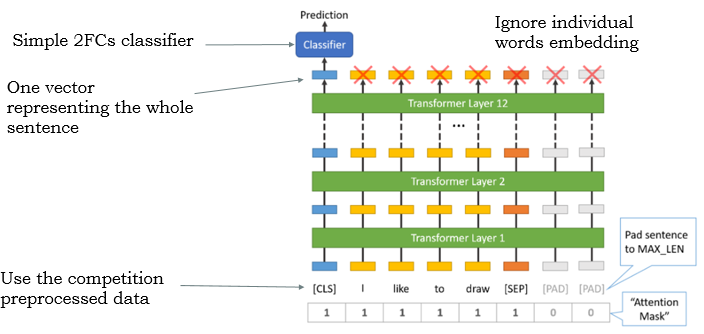
\includegraphics[width=0.999\columnwidth]{Figures/BERTbasedModel.png}}
\caption{BERT-based Baseline Model.}
\label{BERTbasedModel}
\end{figure}

Although BERT is the best possible model known to us, the performance can still be improved by data pre-processing.
So we decided to split the work along two branches, exploring better models, and improving pre-processing of available data while using BERT or BERT like architecture.
We tried bunch of other models such as:
\begin{itemize}
\item Bidirectional LSTMs with pretrained glove model for embedding
\item Using the BERT model itself we also tried bunch of other things such as:
\item Trying a more compact version of BERT (6 layers instead of 12) 
\item Use different pretrained BERT models 
\item Preprocess the data ourselves instead of using the competition pre-processed data
\item Ensemble multiple predictions
\end{itemize}

Furthermore, to improve the obtained performance in the competition, we apply simple ensemble technique by taking the weighted average of our top models predictions. Figure~\ref{EnsempleCoupleOfModels} introduce the diagram for the ensemble technique.   

\begin{figure}[htbp]
\centerline{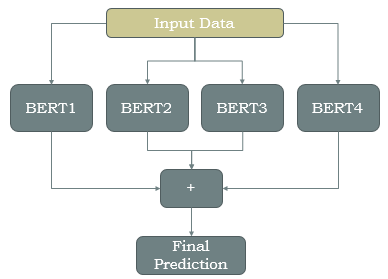
\includegraphics[width=0.999\columnwidth]{Figures/EnsempleCoupleOfModels.png}}
\caption{Ensemple couple of models.}
\label{EnsempleCoupleOfModels}
\end{figure}


\section{Experiments}

\subsection{Dataset}
We based our work on the competition dataset. The primary data for the competition consists of comments classified as toxic or non-toxic (0 and 1). The dataset is divided into train, validation and test splits. The train set’s comments are entirely in english and come either from Civil Comments or Wikipedia talk page edits. The validation and test data's comments are composed of multiple non-English languages\cite{Jigsaw}. They also, include the data from their other competition "Jigsaw Unintended Bias in Toxicity Classification"\cite{Jigsaw2} as an auxiliary dataset, but the dataset has 6 classifications for comments labels instead of just two.

The organizers of the competition provided the dataset in two format; raw text files, and pre-processed data ready for use by BERT models, but they used a small maximum sequence length of only 128 tokens. 

\subsection{Evaluation}

To evaluate a model, depending on the experiment, we may train it on the primary training dataset, auxiliary dataset and validation dataset, but we never let the model train on the test dataset. In fact, the labels for test dataset of the competition are not provided, so the only way to get the score of your model is by submitting the predictions to the competition website. So, that is what we did.

Submissions to the competition are evaluated on area under the receiver operating characteristic (ROC) curve (AUC) between the predicted probability and the observed target. 


  
\subsection{Baseline m-BERT}

For the first experiment, we tried to train our baseline model (the m-BERT-based model) for 5 epochs on the main training dataset and evaluate it on the text dataset. 

After this baseline experiment, we decided to evaluate a more compact version of BERT called DistilBERT with special pretrained weights on multilingual data called distilbert-base-multilingual-cased. This model has only 6 hidden layers instead o the 12 layers by m-BERT. 

We only used one FC layer with one neuron and sigmoid activation function to do the classification. With the memory  limitations on Kaggle environment we adopted this smaller model to be able to add on top of it our own ideas.

Then we investigated improving this model in two directions, one that utilizes the auxiliary dataset for training with early stopping, while the second one only uses the primary dataset.


\subsection{Utilizing The Auxiliary Dataset}

For this experiment, we tried to utilize the auxiliary dataset by converting its labels to be in the range {0,1} by applying a threshold of 0.5 (the recommended threshold from \cite{Jigsaw2} for mapping their labels to toxic and non-toxic). Then we merged this data with the primarily train dataset process it by ourselves with a maximum sequence length of 100 tokens. 

We then trained the model for 10 epochs on the combined training data, and 20 epochs on the validation data while early stopping utilized to stop training whenever the performance on the validation data is not improved after one epoch. 

\subsection{No Auxiliary Dataset}

Without utilizing the auxiliary dataset, with maximum sequence length of 192. Training on the primary dataset for 3
epochs and on the validation dataset for another 3 epochs.

\subsection{Improved Classifier}

Based on previous experiment in this experiment, we increased the maximum sequence length to 120 token (which is still less than the maximum sequence length used in Ep.2.B because processing of the auxiliary dataset requires a lot of memory), and improved the classifier by adding two layers before the final classification layer. The first one, is FC layer with 256 neuron, and ReLU activation function. While the second is a dropout layer with dropout probability of 0.2.

\subsection{Train on Primary and Half The Auxiliary Datasets Separately}

In this experiment we tried to utilize the available memory more efficiently by explicitly releasing any unneeded object. This allowed us to process longer sequences without truncating it. In fact, we changed the maximum sequence length to 250. 

We started, by training on the primary training data for 5 epochs, then process around half of the auxiliary data and train on it for 4 epochs. Lastly, the model is trained on the validation data for 3 epochs before it is used for evaluation. 

\subsection{Train on Primary and Auxiliary Datasets Separately} 

We increased the maximum sequence length to 250 and same setup as Exp.4.A, but after training on half of the auxiliary dataset, we process and train on the other half before training on validation dataset.

\subsection{Ensemble Multiple Predictions}

In this experiment, we take the average of predictions from our top performing models that were trained on both primary and secondary datasets. 

\subsection{Other Failed Experiments}
We tried to implement a Bidirectional Long-Short-Term Memory (BiLSTM) based model with pretrained glove model for embedding, but the experiment failed couple of times. Some of the failures were due to the law speed internet  connection and the fact that we have to use VPN to be able to connect to Kaggle website and run our experiments. In addition, the time limit for the project did not allow us to investigate in all the directions we want, so we focused on BERT-based models.

Furthermore, we tried to use the Off-shelf BertForSequenceClassification to tackle the classification problem but failed for the same above reasons.   

 
\section{Results}
A brief summary of our submissions is presented in Table\ref{ResultsSummary}. As expected we managed to improve the performance as we improve the model and pre-processing. Except for Exp.5.A where training on the whole auxiliary dataset did not  improve the performance, which we think is because the model starts to overfit on it, while it is too different from the training dataset. 

\begin{table}
\begin{center}
\begin{tabular}{|l|c|}
\hline
Implementation	& ROC Score \\
\hline\hline

Baseline m-BERT	& 0.8236    \\
Utilize the auxiliary dataset & 0.8613 \\
No auxiliary dataset	&0.8653 \\
Improved classifier & 0.8782 \\
Primary/$\frac{1}{2}$auxiliary separately & 0.8835 \\
Primary/auxiliary separately & 0.8668  \\
Ensemble multiple predictions & 0.8851 \\
Pre-Trained Transformer [HuggingFace] v2	&0.8782 \\
Pre-Trained Transformer [HuggingFace] v3	&0.8835  \\
Ensemble [m-BERT + Pre-trained] v1 	& 0.9269   \\
Ensemble [m-BERT + Pre-trained] v2 	& 0.9315   \\
Ensemble [m-BERT + Pre-trained] v3 	& 0.9318  \\

\hline
\end{tabular}
\end{center}
\caption{\label{ResultsSummary} Brief summary of our submissions}
\end{table}
Despite the fact that, we are currently ranked as 944 out of 1436 teams, our performance is not very far from the current top team (0.9318 compared to 0.9556). 

\section{Conclusion}

In this work, multiple BERT-based model were successfully implemented to identify toxic comments among text data provided by Kaggle's "Jigsaw Multilingual Toxic Comment Classification Challenge". Finally, we create an ensemble of multiple well performing models and present our results. The reported accuracy of the toxic comment identification by our ensemble is certainly promising and provides a good insight into what to expect when dealing with multilingual data.  

For future work, we may try to use the individual words embedding generated by BERT, and possibly pass them through a couple of Bi-LSTM layers. Furthermore, we may incorporate position embedding to enhance the performance.


{\small
\bibliographystyle{ieee}
\bibliography{egbib}
}

\end{document}
